\chapter{Sequential simulator}
\label{ch:sequential}

\epigraph{The purpose of computation is insight, not numbers.}{Numerical Methods 
for Scientists and Engineers, 1962---Richard Hamming}

In order to begin the implementation of the simulator, an initial version was
considered with the minimum complexity, to verify the correctness of the model.
A graphic subsystem was build with MathGL and OpenGL to produce realtime plots
of different elements of the simulation. Of special interest are the particle
motion, the electric potential and the electric field.

The language of choice was C for the low overhead, the lack of automatic memory
management, the support of different libraries planned in future versions and
the low level design, which allowed us to define most of the data structures
close to the byte level.

\section{Design}

The simulator initially only supported one group of particles of the same charge
and mass, denominated specie. Each particle was implemented as a structure with
a given index $i$, a position vector $\x$, velocity $\v$ and other extra fields
such as the interpolated electric field at the particle position $\E$.
%
Only one dimension was implemented for the first tests, but soon extended to two 
dimensions.  The fields were allocated in contiguous arrays, with the $x$ 
dimension aligned with the cache line, also called row-major storage.

The configuration of the simulation is specified in plain configuration files,
with the syntax defined by the \texttt{libconfig} library. Is important to allow
the user to specify comments in the configuration files, as well as scientific
notation in different values. Additionally, the specification of multiple species
benefits from the sub-configuration block feature, which leads to a more
intuitive representation. The detailed configuration is described in the
chapter~\ref{ch:config}.

The solver used was initially the $LU$ decomposition, used from the $GSL$
numeric library~\cite{gsl}, as the only focus was to obtain valid results, ignoring the
performance. All implementations are tested beforehand with some test cases
designed in \texttt{octave}.

\subsection{Debug mode}

In order to get insight into all the details of the simulation, a mechanism of 
visualization can be very useful: the different fields can be plotted in 
real-time for one and two dimensions, while the particles move around. The 
simulator includes a visualization mode, in which the state of the simulation is 
plotted at a specific period of iterations (by default each iteration is shown).  
In this mode (which we will refer to as debug mode) the simulation is slowed 
down, with a top speed of 60 iterations per second, to follow the visualization 
in the screen.

With this mode activated, the user can observe and quickly check the overall 
behavior of the simulation, as is designed to minimize the delay between writing 
the configuration of the simulation and the execution. Once the simulator is 
running, the user can see several graphs being updated.

The energy measurements are always shown, including potential, kinetic and total 
energy---the total energy must be conserved at all times. In the case of 
one-dimensional simulations, the particles are plotted in the $x$-$v$ phase 
space, with the fields aligned vertically. However, in two dimensions the 
particles are plotted by default in the $x$-$y$ plane which corresponds to the 
physical position in space. The fields now cannot be plotted together, an only 
the electric potential is shown.

\missingfigure{Add some pictures of the simulator in debug mode.}

Once the simulation is properly tested in the debug mode, there is less chance 
that a misconfigured setting ruins a large simulation. This mode has also being 
very helpful when developing the simulator, as several test required to see the 
immediate result of a new feature, or to change a value in the configuration.

\section{Validation}

A set of different tests were designed to determine the correctness of the
simulation.

\subsection{Two particle test}

A simple one-dimensional test consists of two electrons placed at some distance 
different of $L/2$ with no initial speed. The analytical solution is known and 
the motion should follow a harmonic oscillation trajectory. The energy 
conservation can be observed in the figure~\ref{fig:1d-2particles-energy}, where 
the total energy only varies due to the interpolation noise as the time $t$ 
grows in the $x$ axis.
%
\begin{figure}[h]
	\centering
	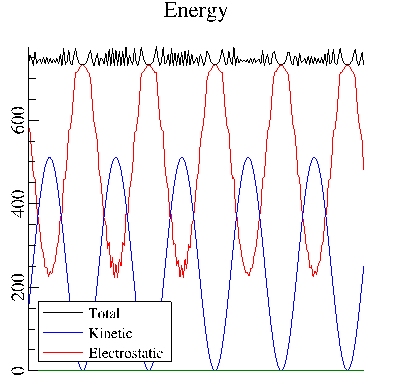
\includegraphics[width=0.4\linewidth]{1d-2particles-energy.png}
	\caption{Energy conservation in two particle test as shown in the simulator 
	(notice the lack of anti-aliasing).}
	\label{fig:1d-2particles-energy}
\end{figure}

\subsection{Two stream instability}

%
\begin{figure}[ht]
	\centering
	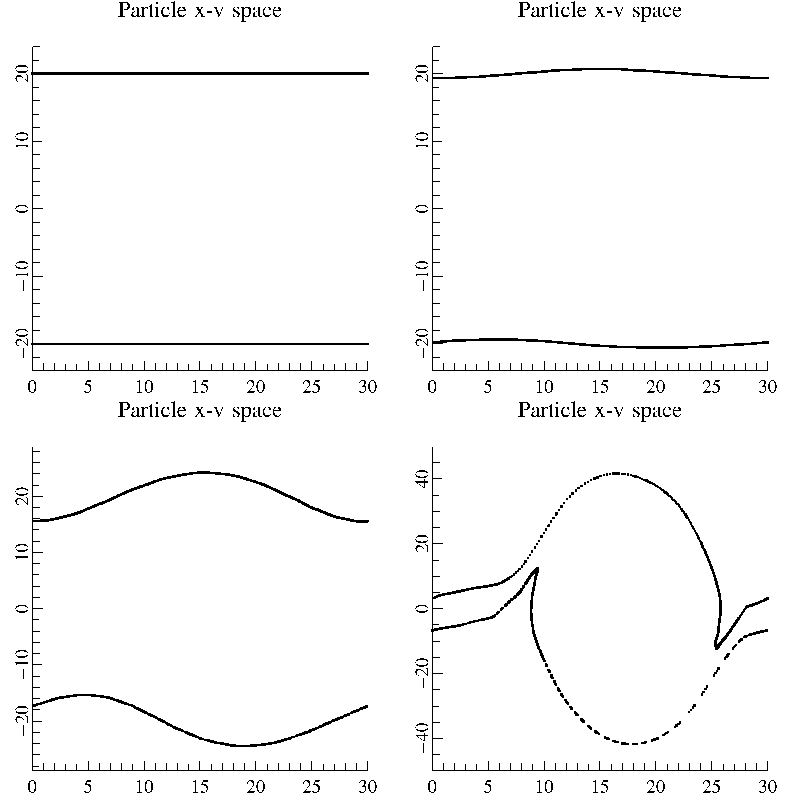
\includegraphics[width=0.8\linewidth]{1d/2stream/out.png}
	\caption{Phase space position--velocity of the two stream instability, shown 
	at iterations: 0, 200, 400 and 600 (left to right, top to bottom)}
	\label{fig:1d-2stream}
\end{figure}

Another example in one dimension is the two stream instability, which consists 
of two streams of particles with opposite velocity. With 500 particles in each 
stream, a very characteristic set of vortices are created in the 
position-velocity phase space, which can be shown in the 
figure~\ref{fig:1d-2stream}.

\subsection{Cyclotron frequency}

In a simulation with two dimensions and a fixed background magnetic field 
$\B_0$, a charged particle with some initial velocity should describe a circular 
orbit. The radius $r_g$ known as the Larmor or gyroradius, can be computed 
analytically as
\begin{equation}
r_g = \frac{m v}{|q| B}
\end{equation}
